\documentclass[border=10pt]{standalone}

\usepackage{tikz}
\usepackage{tikzsymbols}
\usetikzlibrary{calc,patterns,shapes.geometric}

\def\centerarc[#1](#2)(#3:#4:#5){\draw[#1] ($(#2)+({#5*cos(#3)},{#5*sin(#3)})$) arc (#3:#4:#5);}

\begin{document}
	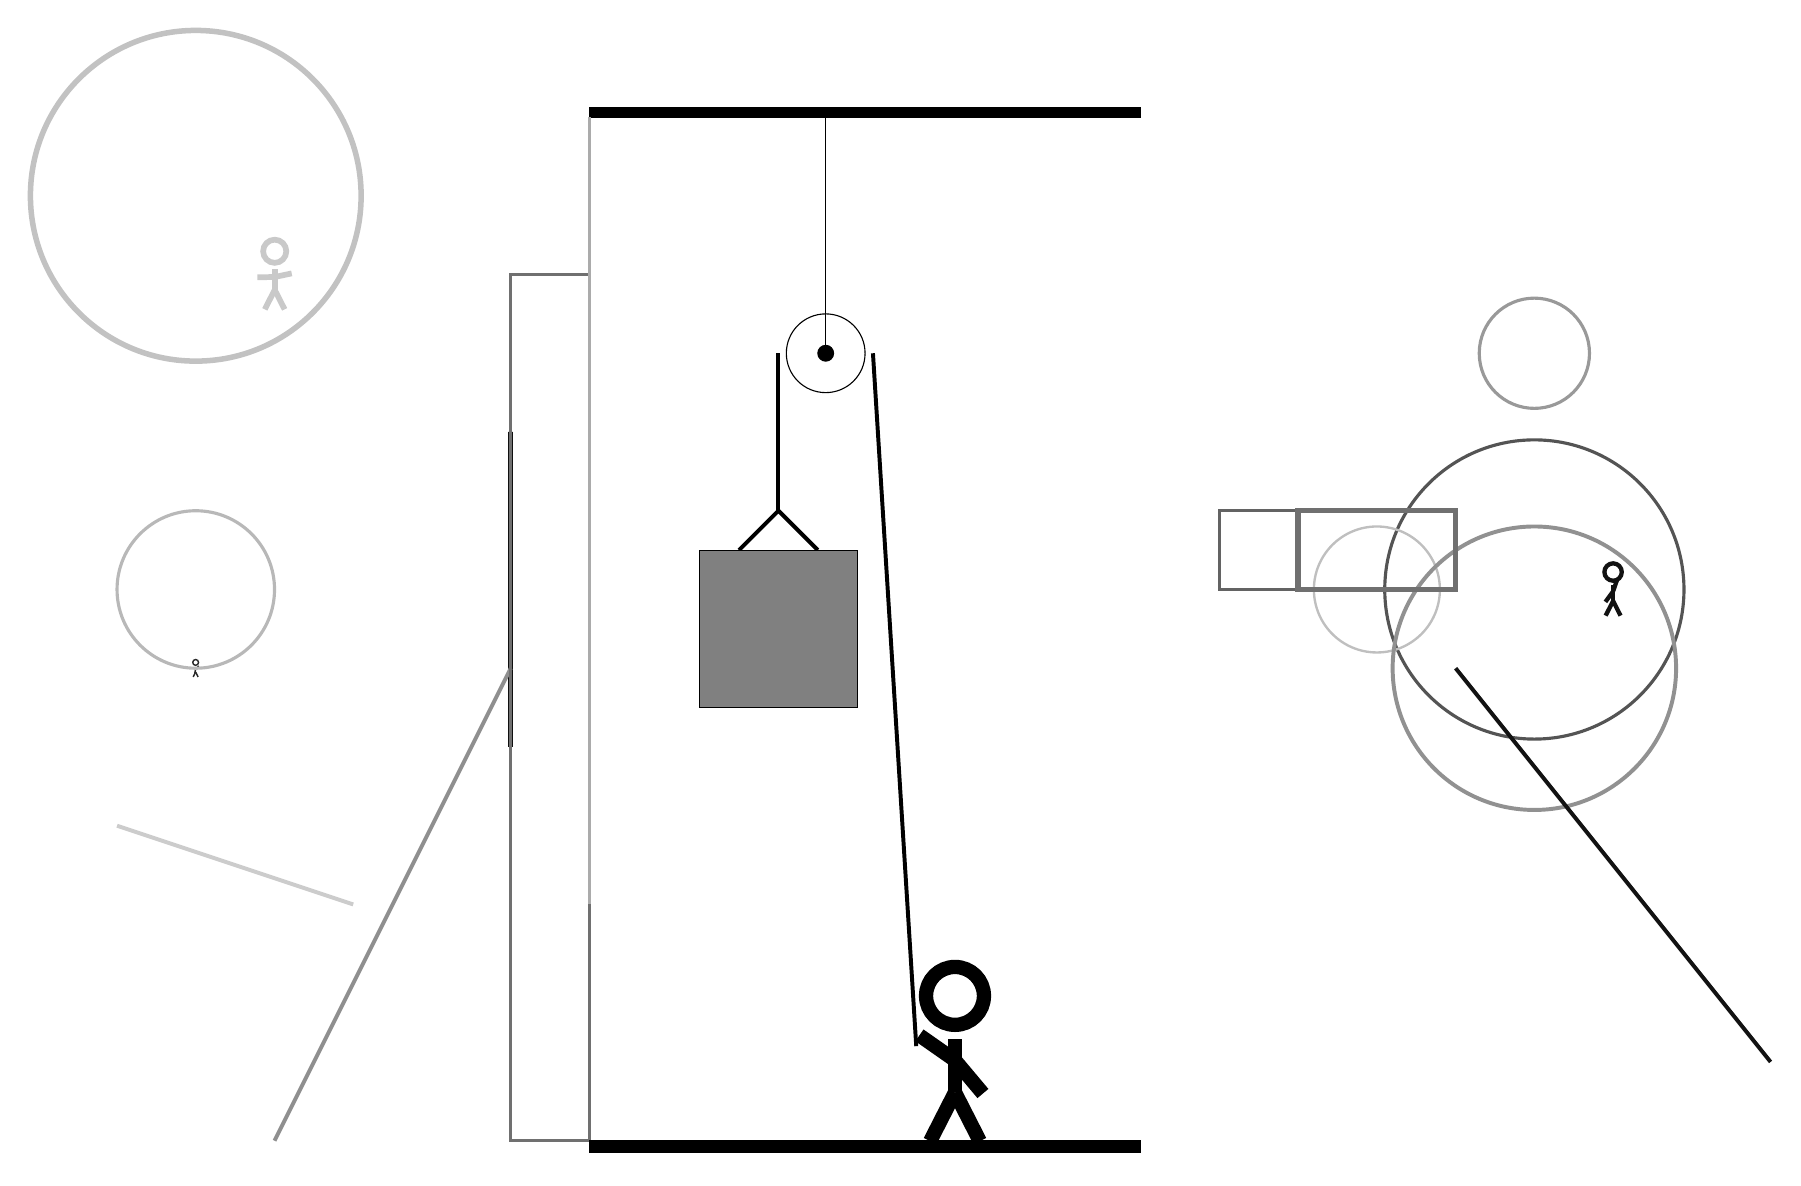
\begin{tikzpicture}
		%%%%% START %%%%%
		
		\draw[fill=black] (-2, 10) rectangle (5, 10.125);
		
		\draw (1, 7) circle (0.5);
		\draw[fill=black] (1, 7) circle (0.1);
		\draw (1, 10) -- (1, 7);
		
		\draw [line width=0.4mm, color=black!67](10, 4) circle (1.9);
		
		\draw [line width=0.3mm, color=black!25](8, 4) circle (0.8);
		\node[line width=0.7mm, color=black!84] at (-7, 3) {\Strichmaxerl[1][79][43]};
		\draw[line width=0.5mm, color=black!20](-5, 0) -- (-8, 1);
		\draw [line width=0.7mm, color=black!24](-7, 9) circle (2.1);
		\draw [line width=0.5mm, color=black!43](10, 3) circle (1.8);
		\draw[line width=0.7mm, color=black!94] (-3, 6) rectangle (-3, 2);
		\draw [line width=0.4mm, color=black!28](-7, 4) circle (1.0);
		\draw[line width=0.4mm, color=black!61] (6, 4) rectangle (7, 5);
		\node[line width=0.5mm, color=black!93] at (11, 4) {\Strichmaxerl[3][54][71]};
		\draw[line width=0.5mm, color=black!44](-6, -3) -- (-3, 3);
		
		\draw [line width=0.4mm, color=black!40](10, 7) circle (0.7);
		\draw[line width=0.4mm, color=black!56] (-3, -3) rectangle (-2, 8);
		
		\node[line width=0.4mm, color=black!21] at (-6, 8) {\Strichmaxerl[4][1][12]};
		\draw[line width=0.5mm, color=black!93](9, 3) -- (13, -2);
		\draw[line width=0.7mm, color=black!56] (7, 5) rectangle (9, 4);
		
		\draw[line width=0.5mm, color=black!33](-2, 10) -- (-2, 0);
		
		\draw[line width=0.5mm] (-0.1, 4.5) -- (0.4, 5.0) -- (0.9, 4.5);
		\draw[fill=black!50] (-0.6, 4.5) rectangle (1.4, 2.5);
		
		\draw[line width=0.5mm] (0.4, 7) -- (0.4, 5.0);
		\centerarc[line width=0.5mm](1, 7)(0:180:0.6);
		\draw[line width=0.5mm](1.6, 7) -- (2.15, -1.8);
		
		\node at (2.6, -1.9) {\Strichmaxerl[10][-35][-50]};
		
		\draw[fill=black] (-2, -3) rectangle (5, -3.15);
		
		%%%%% END %%%%%
	\end{tikzpicture}
\end{document}